\documentclass{article}
%%\usepackage{graphicx}
%%\graphicspath{ {./images/} }

%\usepackage[
  paperheight=8.5in,
  paperwidth=5.5in,
  left=10mm,
  right=10mm,
  top=20mm,
  bottom=20mm]{geometry}
\usepackage[utf8]{inputenc}

%%\usepackage{biblatex}
\usepackage{graphicx}
\usepackage{wrapfig}
\usepackage[bottom]{footmisc}
\usepackage{listings}
\usepackage{enumitem}

\usepackage{wrapfig}
\usepackage{ragged2e}

\usepackage{array}
\usepackage[table]{xcolor}
\usepackage{multirow}
\usepackage{booktabs}
\usepackage{hhline}
\definecolor{palegreen}{rgb}{0.6,0.98,0.6}

\usepackage{amsmath}
\usepackage{amssymb}
\usepackage{multicol}
\usepackage{lipsum}
\usepackage{hyphenat}
\PassOptionsToPackage{hyphens}{url}
\usepackage{url}

\usepackage{rotating}

\usepackage{pdfpages}

%% support use of straight quotes in code listings
\usepackage[T1]{fontenc}
\usepackage{textcomp}
\usepackage{listings}
\lstset{upquote=true}

%% for shrinking space between lines
\usepackage{setspace}

\usepackage{caption}

\newcommand*{\affaddr}[1]{#1} % No op here. Customize it for different styles.
\newcommand*{\affmark}[1][*]{\textsuperscript{#1}}
\newcommand*{\email}[1]{\small{\texttt{#1}}}
\newcommand{\tarot}{\textsc{Tarot}}
\renewcommand*\contentsname{\centering Table of Contents}

\renewcommand{\footnoterule}{%
  \kern -3pt
  \hrule width \textwidth height 0.5pt
  \kern 2pt
}

\usepackage{titlesec}
\titleformat*{\section}{\large\bfseries}
\titleformat*{\subsection}{\normalize\bfseries}
\titleformat*{\subsubsection}{\normalize\bfseries}

% define variables
\newcommand{\confOrdinal}{34th}
\newcommand{\confName}{South Central}
\newcommand{\confDates}{March 31st}
\newcommand{\confYear}{2023}
\newcommand{\confSchool}{Stephen F. Austin State University}
\newcommand{\confCity}{Nacogdoches, TX}
\newcommand{\journalVolume}{38}
\newcommand{\journalNumber}{7}
\newcommand{\journalMonth}{April}
\newcommand{\journalYear}{2023}
\newcommand{\regionalEditor}{Mustafa Al-Lail}
\newcommand{\regionalEditorSchool}{Texas A\&M International University}



\title{Developing Incident Response-Focused Cybersecurity Undergraduate Curricula 
\footnote{\protectCopyright \copyright \confYear\ by the Consortium for Computing Sciences in Colleges.
Permission to copy without fee all or part of this material is granted provided
that the copies are not made or distributed for direct commercial advantage,
the CCSC copyright notice and the title of the publication and its date appear,
and notice is given that copying is by permission of the Consortium for
Computing Sciences in Colleges.  To copy otherwise, or to republish, requires
a fee and/or specific permission.

}
}

% Target typesetting:
%
%  Baochuan Lu, Author A, John Meinke, Author B
%        Computer and Information Sciences
%          Southwest Baptist University
%               Bolivar, MO 65613
%            {blu,author}@sbuniv.edu
%          Computer Science Department
%              Another University
%              Our Town, TX 00000
%           {jmeinke,author}@univ.edu

\author{
Junghwan ``John'' Rhee, Myungah Park, Fei Zuo, Shuai Zhang, \\
Gang Qian, Goutam Mylavarapu, Hong Sung, Thomas Turner\\
Department of Computer Science\\
University of Central Oklahoma\\
Edmond, OK 73034\\
\email{\{jrhee2,mpark5,fzuo,szhang10,gqian,smylavarapu,hsung,trturner\}@uco.edu}\\
%\affmark[2]Computer Science Department\\
%Another University\\
%Our Town, TX 00000\\
%\email{\{jmeinke,author\}@univ.edu}\\
}

\begin{document}
\maketitle

\begin{abstract}
Increasing cybersecurity incidents call for a competitive cybersecurity workforce more than ever. We create new comprehensive cybersecurity university curricula in a metro undergraduate-focused regional university. Our program is distinguished from other programs by specializing in incident response, which addresses the analysis of attack trails and damages followed by infrastructure hardening including software, systems, and policies to prevent future attacks. This special theme requires practical strength such as certifiable deep knowledge, hands-on skills, and research-involved cybersecurity activities. We present the design and implementation of the cybersecurity curricula in our institution.
\end{abstract}

\section{Introduction}

Increasing cybersecurity incidents and malware hits as seen in the Colonial pipeline incident \cite{colonial} have been issues with real impact on our society. Reputable sources such as Cyberseek~\cite{cyberseek} and ISC$^2$~\cite{isc} from industry leaders estimate 4.7 million cybersecurity experts are lacking. Cybersecurity is becoming increasingly important in computer science education as an essential skill because a poor design without careful consideration of software vulnerabilities and attack surfaces can invite adversaries and incidents in no time in the current connected world. This trend is evidenced by multiple movements of integration of cybersecurity into the design and development of software such as Microsoft's Secure Software Development Life Cycle (SDL)~\cite{sdl}. Recent announcements promoting memory-safe languages as a major transition by Microsoft and NSA show cybersecurity is an inseparable subject in computer science education and affects the major decision in computing.

%Our computer science department has ABET-accredited regional programs. 
%We also created a software engineering program which is one of the first programs specializing software engineering in computer science. 
As cybersecurity has been a major social issue with great demand in the workforce, our department created a new cybersecurity program specialized in incident response, which is an essential subject for cybersecurity analysts who are the experts to evaluate and improve each organization's cybersecurity status.
%
This paper proposes a new design of cybersecurity education curricula with the following contributions:

\begin{itemize}
    \item We introduce a design of an undergraduate cybersecurity program specialized in incident response.
    
%    \item Introduction of a cybersecurity program with the consideration of multiple aspects of students' career
    
    \item We present a case study of the design and implementation of this program as a real instance of an incident response-focused cybersecurity program in a regional university.
    
\end{itemize}

We present the design of our curricula in Section \ref{sec:design}.
%The design and implement are presented in Section \ref{sec:design}. 
%We present the evaluation in Section \ref{sec:evaluation}. 
Related work is discussed in Section \ref{sec:relatedwork}. We discuss our plan for the next step in Section \ref{sec:discussion}. Our paper is concluded in Section \ref{sec:conclusion}.

\section{Design of Incident Response-focused Curricula}
\label{sec:design}


We set multiple objective requirements for the design of our cybersecurity program to make it distinguished from others.

\begin{figure}[t]
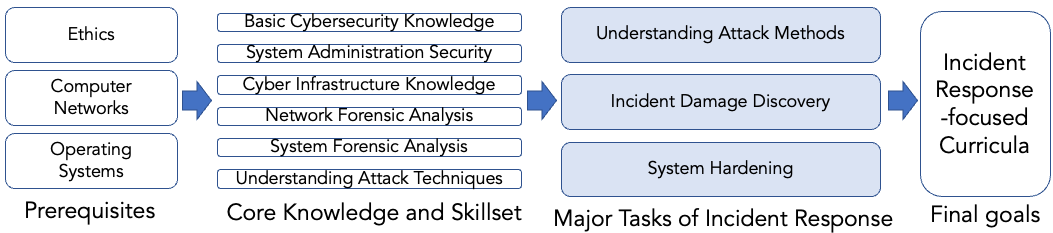
\includegraphics[width=\textwidth]{2648_1.png}
\centering
\caption{Mapping goals with major tasks, core knowledge, and prerequisites.}
\label{fig1}
\end{figure}

\subsection{Design Requirements}

\begin{itemize}
    
\item \textbf{R1: Specialized education plan for unique competitiveness:} First, we wanted to make our program unique and distinguished with a unique value in incident response. This requirement can be fulfilled by understanding the necessary skill sets and corresponding course design. Figure \ref{fig1} presents the mapping that we determined. Core skillsets to conduct incident response include an understanding of cybersecurity attack methods, assessment of attack damages, and system hardening methods to prevent future attacks. We determined the required core skills and knowledge to perform these tasks and support prerequisites.

\item \textbf{R2: Multiple cybersecurity education targets:} Second, our computer science department has students with multiple different degree interests such as B.S. of Computer Science, B.S. of Software Engineering, B.S. of Data Science, and M.S. of Computer Science. Cybersecurity curricula should be positioned to be beneficial to students who need cybersecurity with different degree goals.


\item \textbf{R3: Quality hands-on skills:} 
Cybersecurity employees require strong knowledge and hands-on skills which help them to become effective employees in their tasks investigating incidents and securing the infrastructure which require strong underlying system knowledge. 
%For a strong program, it is an important design decision.

\item \textbf{R4: Credentials to strengthen job applications:} 
The current competitive job market often calls for cybersecurity credentials in job applications. For fresh graduates who start the first position in their job career, this is an important aid to assist their landing positions.
%The second group will have a job in non-cybersecurity positions. 
%As cybersecurity becomes increasingly important this is a topic that should be cared about by all students.

\item \textbf{R5: Research experience:} Participating in research provides an opportunity to learn the latest technology, challenges, and solutions. Tackling and solving unsolved problems could nurture students as problem solvers. Also for students who seek research career paths, research experience will become an important record to help their applications.

\end{itemize}

\subsection{Design Foci of the Proposed Program}
With these requirements in mind, we designed our curricula to satisfy each of the requirements.



\begin{figure}[th]
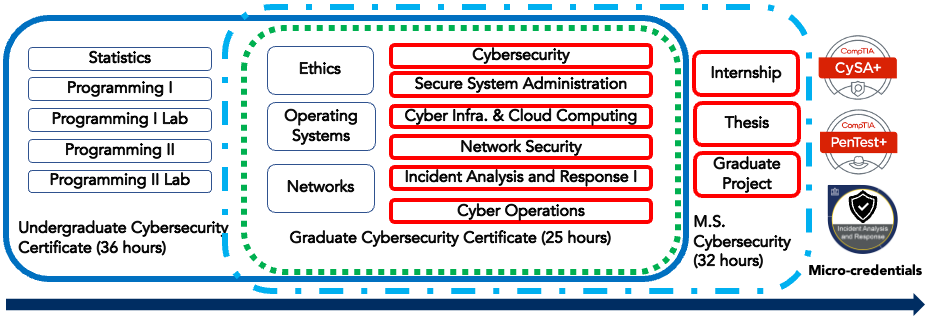
\includegraphics[width=\textwidth]{2648_2.png}
\centering
\caption{Curricula of proposed courses, degrees, and certificates.}
\label{fig2}
\end{figure}

\begin{itemize}

\item \textbf{D1: Focus on incident response:} Our department has multiple faculty members working on cybersecurity. Based on their research and teaching background, we designed and implemented cybersecurity curricula specializing in incident response, as shown in Figure \ref{fig2}. The required knowledge and skillset shown in Figure \ref{fig1} are fulfilled by six cybersecurity core courses and three supporting courses. We created an undergraduate certificate that provides comprehensive cybersecurity skillsets with these courses. We are also creating graduate-level programs for students who seek advanced study.

\item \textbf{D2: Multiple student targets:} We set two types of student targets for our education program: The first target is the frontline of cybersecurity defense. The students of this group intend to work in the cybersecurity positions such as cyber analysts, penetration testers, and cyber operators. The second education target is the computer science majors with cybersecurity awareness and competitiveness.  For the second group, our program is positioned to provide strong add-on cybersecurity skills for their main career goals to make them more competitive.      

\item \textbf{D3: Combination of hands-on skills and deep knowledge:} Hands-on assignments and projects provide an opportunity to deeply understand the learning materials and apply what they have learned into practice. We train our students to be competitive in skills as well as knowledge so that their capabilities are practical and influential in their positions. 
%
For instance, the Secure System Administration course teaches essential utilities, command line interfaces, and scripting (bash, PowerShell) based on Windows and Linux virtual machines. The Incident Analysis and Response I course covers the collection of operating system data and their investigation. Students analyze the data using various UNIX tools and scripting to understand attack details and make an incident report. The Cyber Operation course teaches penetration testing to discover the weaknesses of systems and software using a comprehensive set of tools. Also, students participate in multiple catch-the-flag (CTF) events  with the instructor and experience vulnerability discovery in the field.

\item \textbf{D4: Cybersecurity credentials:}
%Competitive job markets call for credentials in students' job applications. For undergraduate graduates who start the first step in their job career, this is an important aid to assist their landing positions.
Our department became a partner of CompTIA~\cite{comptia}, which is a well-known cybersecurity organization in the industry and government. Our curriculum is closely aligned with its certificates.
Besides, in several courses, we introduced
micro-credentials that can be validated regarding the details of skills obtained.
We also are preparing applications for accreditation such as NSA National Centers for Academic Excellence in Cybersecurity~\cite{cae}.

\item \textbf{D5: Research-involved education program:} Our department has multiple faculty members who are active in cybersecurity research. We offered multiple research assistant opportunities almost every semester providing research experience. Their work is submitted to research publications and research events such as Oklahoma Research Day.

\end{itemize}

%\section{Implementation}
%\label{sec:implementation}

\subsection{Degrees and Certificates}

We created multiple cybersecurity programs as follows.

\begin{itemize}
    \item \textbf{Undergraduate cybersecurity certificate}: Undergraduate level cybersecurity certificate is offered to the students who complete a list of core subjects in cybersecurity and supporting courses. This certificate will provide a cybersecurity credential for undergraduate students (D2).



\item \textbf{Micro-credentials:} Multiple courses offer micro-credentials for their successful completion. These are issued using a third-party service called ``Credly'' so that a digital certificate can show the details regarding the earned skill (D4) by following the URL links assigned to the issued micro-credentials.

\item \textbf{M.S. in Cybersecurity:} We submitted an application for a new Master's degree in Cybersecurity to provide advanced education for students who seek the next level. Currently, it is in the review process.

\item \textbf{Graduate cybersecurity certificate:}
We also submitted an application for a graduate-level cybersecurity certificate to provide a cybersecurity credential without the full commitment of the master's degree due to work and other reasons. This is also under review.



\end{itemize}




\subsection{Cybersecurity Courses}

We offer multiple courses specialized in cybersecurity in our department.


\begin{itemize}

    \item \textbf{Cybersecurity:}
This course introduces the foundations of cybersecurity. The course topics include cyber threats, security principles and goals, security policies and mechanisms, access control, cryptography, operating system and software security, and legal and ethical issues in cybersecurity. 

    \item \textbf{Network Security:}
This course introduces the principles of network security, which covers network security policy, packet filtering, firewalls, port scanning, intrusion detection and prevention systems, virtual private networks, DNS security, host hardening, and network incident response.

    \item \textbf{Secure System Administration:}
This course introduces the essential knowledge and skillsets for system administration. Students will learn  hands-on system administration techniques including scripting, shells, editors, utilities, policies, regulations, and risk management (D3). 

    \item \textbf{Incident Analysis and Response I:}
This course introduces the knowledge and skillsets for incident response, system analysis, and security controls. Students will learn hands-on techniques to investigate the symptoms of attacks and perform a comprehensive analysis to discover the details of attack damages,  recover the systems, and protect them from future attacks. 
%Also, students will become familiar with core security concepts for incident analysis and response, such as vulnerabilities, cyber kill chain, threat intelligence, and indicators of compromise (IOC).
This course covers the materials for the CompTIA CySA+ certificate (D1, D3, D4).

    \item \textbf{Cyber Operations:}
This course introduces  techniques and hands-on experiences in penetration testing, software security, and cyber operations. Students will learn vulnerable/secure code patterns, vulnerability types, and security frameworks for vulnerability testing. This course covers the materials for the CompTIA PenTest+ certificate (D3, D4).

    \item \textbf{Cyber Infrastructure and  Cloud Computing:}
This course introduces the technologies of cloud computing, the stack of cloud service models, and the design of cloud-based applications. Hands-on studies over prevailing cloud services are provided to illustrate the common components, interfaces and practices for resource management and application development at scale.

\end{itemize}

\subsection{Extra Activities}

In addition to the presented curricula, we created several supporting activities and groups to enhance cybersecurity education.

\begin{itemize}

\item \textbf{Cybersecurity Center:} We established a cybersecurity center, which serves as a hub for cybersecurity activities at our institution (D5).

\item \textbf{Cybersecurity Research Groups:} Our faculty members run research labs to lead cybersecurity research and educational projects with undergraduate and graduate students (D5).

\item \textbf{Cybersecurity Community Activities:} We are participating in multiple cybersecurity community activities such as Catch the Flags (CTF) events. We are also collaborating with  industry and government organizations forming an advisory board.

\end{itemize}

%\section{Evaluation}
%\label{sec:evaluation}

\section{Related Work}
\label{sec:relatedwork}

There are multiple papers regarding the design of cybersecurity curricula and the survey of cybersecurity programs related to this paper.

\textbf{Design of Cybersecurity Curricula:}
%
Santos et al.~\cite{7918179}
present the reflections regarding the curricula contents to be considered to design a graduate-level curriculum in cybersecurity.
%
In \cite{6573305}, Schneider et al. argue the issues about what should be taught and which are not well addressed by many of the university cybersecurity faculty.
%
Rowe et al.~\cite{10.1145/2047594.2047628} discussed 
 the role of cybersecurity in an IT education context and argue why IT programs should champion this topic. 
 %The relationship between Information Assurance and Security as a currently recognized discipline within IT and advanced cyber-security topics are presented. 
%
Rashid et al.~\cite{8395134}
present the Cyber Security Body of Knowledge (CyBOK) project that classifies the foundational and generally recognized knowledge on cybersecurity.
%
Blaken-Webb et al.~\cite{blanken2018case}
describe the rationale for and implementation of an experimental graduate-level cybersecurity ethics course curriculum recently piloted at their school.
%
Blair et al.~\cite{8677338} present a vision and curricula for multi-disciplinary cybersecurity teams which are made up of experts of diverse abilities and expertise.
%
%\cite{10.1145/2325296.2325367} presents a new cybersecurity course that is required and taken by 600 first-year students in the United States Naval Academy. It describes the challenges such as finding qualified staffs and resouces.
% 
Yuan et al.~\cite{8252239} provide a detailed account of designing and developing a hands-on cybersecurity project, which consists of penetration testing, defending an enterprise-level network system, and performing a comprehensive IT audit.
%
The authors of \cite{6759208}
 propose a course of study in cybersecurity designed to 
 target homeland security students.
 The curriculum promotes the intellectual strengths of students in this discipline and that is consistent with the broad suite of professional needs.
%
Saharinen et al.~\cite{10.1145/3369255.3369266}
 describe a model for designing a degree program in cybersecurity. The authors establish the guiding frameworks and requirements within the European Union for a degree program.  
%
Sharevski et al.~\cite{8340471}
 developed an interdisciplinary course for learning in the fields of cybersecurity and interaction design. The inaugural course teaches students secure user interface design.
%
Yue et al.~\cite{10.5555/3532930.3532933}
present a case study of an ABET-accredited cybersecurity program. %We are preparing for the accreditation from NSA National Centers of Academic Excellence in Cybersecurity (CAE) \cite{cae} currently.
%
Luallen et al.~\cite{6480056}
 discuss the development of a course and laboratory environment regarding an undergraduate and graduate-level critical infrastructure and control systems cybersecurity curriculum.

While there have been multiple approaches proposed for cybersecurity curricula, our proposal is differentiated from them because it is a cybersecurity education program with a specialty in incident response education for undergraduate students.


\textbf{Survey of Cybersecurity Education Programs:}
There are prior surveys on cybersecurity education programs.
Multiple researchers~\cite{CABAJ201824,CHOWDHURY2021100361,inbook,9042416,8688137}
 present an overview and comparison of existing curriculum design approaches for cybersecurity education as a survey and review.
%Cabaj et al.~\cite{CABAJ201824} present guidelines used to analyze and review 21 cybersecurity master programs, focusing on the contents of their courses, structure, admission requirements, duration, requirements for completion, and evolution.
%
%Chowdhury et al.~\cite{CHOWDHURY2021100361} conducted 
%a systematic literature review with the purpose of investigating and analyzing key competencies and skills required for cybersecurity in critical infrastructure.
%
%Pencheva et al.~\cite{9042416} present a series of consultation and survey work from educators and other participants on what cybersecurity knowledge should be brought into secondary schools of ages 12-16.
%This article focuses on the U.K. context only, yet the findings can have relevance in other similar contexts worldwide as the shortage of cybersecurity workers is an inter- national and pressing issue.
%Our analysis of the workshop transcript materials revealed two key findings.
%
%Ruiz et al.~\cite{8688137} surveyed 100 computer science undergraduate courses in the UK to determine the capabilities to write secure software. 
%
Yamin et al.~\cite{10.1145/3339252.3340527}
aim to identify commonalities in skillset requirements for multiple cybersecurity roles like penetration tester, security operation center analysts, digital forensic and incident responders, and information security managers. They determined five main domains which are all included in our curriculum.


%\cite{10.1145/3328778.3366878} presents a study where high school students were taught computing and cybersecurity concepts using a hands-on robotics platform.




%\cite{crumpler2019cybersecurity}





%The authors of \cite{10.1145/3197091.3197110} present the design of an undergraduate course and cybersecurity learning modules that fit into the liberal arts education. 

\textbf{Cybersecurity Education Framework:}
NIST's NICE framework \cite{6226542} 
aims to create an operational, sustainable, and continually improving program for cybersecurity awareness, education, training, and workforce development that advances the US’s long-term cybersecurity posture. This framework provides a foundation for most cybersecurity education programs.








 
%\cite{10.1145/2538862.2538990} reports the discussion result of a workshop hosted by the ACM Education Board with funding by the National Science Foundation. It includes the major points and challenges discovered from the workshop participants.  

% book review
%\cite{1236229}





\section{Discussion}
\label{sec:discussion}

This paper presents the design and implementation of our cybersecurity program. After its long-term operation for multiple years, we plan to publish the outcome of our program and reflection on the result including further enhancement, modifications, student career, and lessons from the operation as future work.

\section{Conclusion}
\label{sec:conclusion}

We propose cybersecurity curricula focused on the incident response which is an essential task for cybersecurity workforce to address security incidents and secure infrastructure. We designed the curricula by determining core knowledge and skillset for the major tasks of incident response and then mapping them to six core cybersecurity courses. Our institution implemented this design and offers an undergraduate cybersecurity certificate. In addition, currently, we are in the process of creating a graduate-level master's degree and cybersecurity certificate as advanced steps. We hope our design and experience could be helpful to the institutions that plan a new cybersecurity program.


\medskip

\bibliographystyle{plain}
\bibliography{2648}

\end{document}
